% *****************************************************************************
% * Copyright (c) 2007 by Elexis
% * All rights reserved. This document and the accompanying materials
% * are made available under the terms of the Eclipse Public License v1.0
% * which accompanies this distribution, and is available at
% * http://www.eclipse.org/legal/epl-v10.html
% *
% * Contributors:
% *    G. Weirich - initial implementation
% *
% *  $Id: settings.tex 4904 2009-01-03 17:58:33Z rgw_ch $
% *******************************************************************************
%
% !Mode:: "TeX:UTF-8" (encoding info for WinEdt)

\label{settings}
Tout les réglages se trouvent dans le même dialogue sous \textsc{fichier-options}  (Fig. \ref{fig:settingsmain}).
%\usepackage{graphics} is needed for \includegraphics
\begin{figure}[h]
\begin{center}
  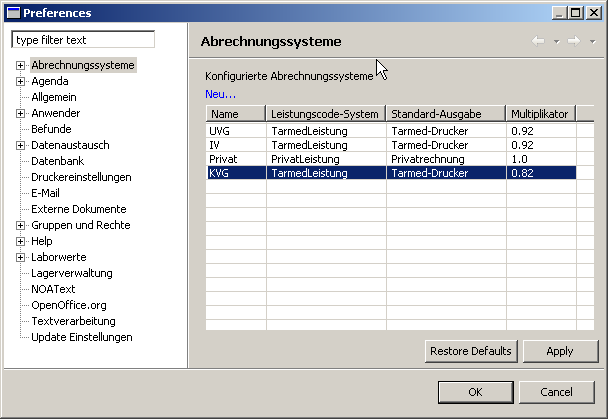
\includegraphics[width=0.6\textwidth]{images/settingsmain}
  \caption{Einstellungs-Dialog}
  \label{fig:settingsmain}
\end{center}
\end{figure}


Comme d'habitude dans Elexis le contenu de ce dialogue est dépendant des Plugins installés. Les onglets, qui se trouvent du côté gauche, permettent de choisir le domaine pour lequel on voudrait changer les réglages. Nous parlons ici que des domaines qui appartiennent à l'installation de base de Elexis. Normalement tout les réglages de base qui se trouvent dans le  \glqq paquet d'installation de base\grqq{}devraient être arrangés de façon qu'en principe il n'y faudra pas faire d'adaptation. Pour cette raison il n'est pas indispensable que vous lisiez ce chapitre.

\section{Systèmes de facturation}
\label{settings:abrechnungssystem}
\index{Système de facturation}
\index{LAMAL}\index{LAA}\index{TarMed}
Sur cette page vous définissez le type de système de facturation que vous utilisez dans votre cabinet. 

Etant donné qu'Elexis est un logiciel universel qui ne soutient pas seulement des médecins mais aussi d'autres professionnels dans le système de santé, le système de facturation est tenu de façon très ouverte. Ceci implique la nécessité d'une configuration initiale.

La comptabilisation des prestations implique trois éléments de base :
\begin{enumerate}
    \item Un système de codification. Expliqué de façon simplifiée, il s'agit d'un concept qui permet de nommer chaque prestation et de lui attribuer une valeur comme par ex. sous \glqq Tarmed\grqq{}, \glqq Tarif d'acupuncture \grqq{} etc.
   \item Un concept des garants : il s'agit donc de savoir qui reçoit la facture et qui paye finalement.  Par ex. : Tiers Garant, Facture en privée etc.
   \item Un concept de facturation : Comment la facture doit-elle être établie et comment doit-elle être envoyée ? (électroniquement, sur papier ?)
\end{enumerate}

Un ensemble d'un système de codification, d'un concept concernant le garant et un concept de facturation nous appelons un  \glqq système de facturation\grqq{}.

Elexis permet de définir ad libitum multiples systèmes de facturation qui peuvent exister parallèlement et qui peuvent être utilisés selon besoin. 

Chaque système de facturation à ses propres qualités :\\
\begin{wrapfigure}{l}{5cm}
    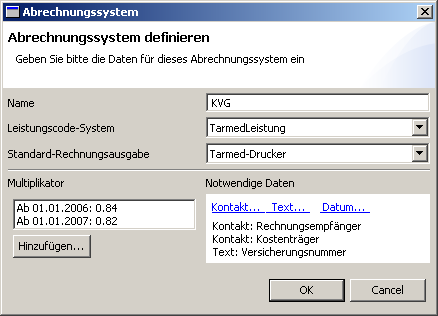
\includegraphics[width=4.7cm]{images/abrechnungssystem1}
    \caption{Abrechnungssystem Detail}
    \label{fig:abr1}
\end{wrapfigure}

Le nom peut être choisi librement, le système des codes de prestation et la facturation standard peut être choisi selon les Plugins installés. (Pour des systèmes de facturation qui n'existent pas encore il faudra produire des Plugins.) Le multiplicateur est un facteur qui est appliqué pour chaque prestation qui sera comptabilisée. On pourra donc utiliser des différents systèmes de facturation avec le même système des codes de prestation mais avec des différents multiplicateurs  (\glqq point de taxe\grqq{}). Avec\textit{ajouter} vous pouvez définir un multiplicateur qui sera valable à partir d'une date spécifique.

Finalement, dépendant du système de facturation vous nécessitez des différents données pour pouvoir facturer des prestations. Il s'agit par ex. du récepteur de la facture, du garant, numéro etc.
Elexis ne donne pas de directives en ce qui concerne ceci. Vous pouvez introduire tout ce que vous voulez. Les différents types de données sont possibles : Texte, contacte et date. (Dans le cadre de l'assurance accident LAA par ex. aussi la \glqq date de l'accident\grqq{}).\\


\section{Général}
Sur cette page sont définis tout les réglages généraux pour le fonctionnement du logiciel.
Il s'agit des :
\subsection{Réglages pour le log}
Le \glqq Log\grqq{} est le journal de bord d'un logiciel dans lequel des différentes informations qui concernent le déroulement du logiciel se trouvent stockées et qui pourront par exemple être utiles pour une recherche de faute.
\begin{itemize}
  \item Fichier journal : Endroit où sont stockés les informations du 'log'. Normalement ceci devrait être le fichier  \glqq elexis.log\grqq{} qui se trouve dans votre répertoire des données.  La valeur \glqq none\grqq{} n'est utile que lorsque vous démarrez Elexis depuis un environnement de développement.
  \item Grade du log : Combien de messages doivent être émis. Au grade 1 seront émis seulement des messages concernant les fautes les pires qui demandent par exemple un arrêt du logiciel. Au grade 5 seront émis et notés dans le Log, beaucoup de messages qui ne seront utile que dans des cas très spécifiques. Nous suggérons pour l'activité normale le réglage d'un grade 2 ou 3.
  \item Grade d'alerte : Des messages qui ont un certain degré d'importance ne seront pas seulement notés dans le fichier journal (Log) mais seront montrés directement sur l'écran. Attention ! Si vous choisissez un grade d'alerte trop haut, vous serrez tout le temps dérangé  par des boxes de popup. Nous recommandons un grade 1.
  \item Nom de la table pour Trace : Trace signifie que toutes les actions seront enregistrées dans un tableau spécifique. A l'aide de ce tableau on pourra plus tard constater de quel poste de travail à quel moment quel action avait été exécutée par Elexis. Cela permet un contrôle très exact des opérations mais aux dépens de la rapidité de travail et de la capacité de stockage. Nous conseillons normalement le réglage \glqq none\grqq{}.
  \item Langue favorisée : Ce réglage ne définit pas dans quelle langue Elexis sera utilisé (Ceci est déterminé par les paramètres du système d'exploitation ou si jamais par les paramètre de démarrage), mais plutôt quelles versions de Tarmed ou CIM-10 seront importées.
  \item Durée de stockage dans le cache : Ceci est un réglage très technique. Il s'agit de déterminer combien de temps des objets de provenance de la base des données resteront valable avant qu'une nouvelle lecture sera nécessaire. S'il y a plusieurs postes de travail dans le réseau vous devrez choisir de préférence un temps court (par ex. 5 secondes) mais si vous voulez accéder à Elexis depuis chez vous à l'aide d'un raccordement Internet lent, il vaudra mieux de choisir un temps prolongé (par ex. 300 sec.).
  \item Intervalle de mise à jour : Après combien de temps Elexis doit actualiser les 'Views'. Lorsque par exemple l'assistante met pour un patient le signe \glqq arrivé\grqq{} dans l'agenda il faudra attendre le temps introduit par secondes jusqu'à ce que vous voyez sur votre écran ce changement de status. Si vous introduisez un délai trop court, la charge pour le réseau devient inutilement importante.
\end{itemize}
\section{Utilisateur}
Dans ces paramètres se trouvent des réglages qui sont spécifiques pour l'utilisateur. Si vous préférez un réglage homogène, vous pouvez sauvegarder un réglage spécifique sous un nom spécifique et le télécharger depuis un autre compte d'utilisateur ou un autre poste de travail.

Les boutons  \glqq télécharger le réglage depuis \ldots\grqq{} respectivement \glqq sauvegarder réglage sous\ldots\grqq{} concernent les réglages individuels d'un utilisateur (en principe tout ce qui se trouve dans la branche \textsc{utilisateur} des réglages). Tandis que les boutons \glqq Paramètres de travail  \ldots\grqq{} concernent les réglages de perspectives de mise en page qui sont stockés sur le poste de travail spécifique.

\subsection{Utilisateur - Aperçu}
\label{userconfig}
Plusieurs options d'affichage s'y trouvent :
\begin{itemize}
\item Champs extensibles : il s'agit des champs qui peuvent êtres ouverts et qui se trouvent dans certaines 'Views' comme par exemple dans la View 'Données-Patient-Détail' où on peut ouvrir le champ 'Diagnostic' ou 'Remarques' etc. Vous pouvez définir si ces champs doivent être toujours ouverts ou toujours fermés lors du premier accès ou si le système mémorise toujours le dernier état.
\item Champs à afficher dans la liste des patients : Ceci définit les champs de filtrage à l'aide de lesquels on peut chercher un patient dans la liste des patients. Normalement le nom, prénom et date de naissance sont proposé comme critères de filtrage mais on peut par exemple aussi laisser afficher le numéro de patient.

\item Champs supplémentaires sur la feuille détaillée du patient: Vous pouvez introduire ici par un texte supplémentaire n'importe quelle information que vous voulez pouvoir saisir pour vos patients et qui ne peut pas être saisi sous 'remarques' ou par une 'étiquette'. Introduisez simplement par ligne un nom qui désigne le type de donnée à sauvegarder.

\end{itemize}

\subsection{Utilisateur - Police de caractères}
Ici vous pouvez définir pour tout les 'Views' le type et la taille de police d'écriture. Certains Views et Plugins peuvent toujours encore définir d'autres polices d'écriture mais ceci est le réglage standard. 

\section{Echange des données}
Ceci est une catégorie collective pour le réglage des Plugins qui permettent le transfert des données depuis Elexis vers l'extérieur mais aussi le transfert de l'extérieur vers Elexis. Il dépend entièrement du Plugin de transport installé quelle page d'accueil vous sera présentée. 
\section{Base de données}
Affiche les détails des réglages des liens avec la base de données. 
\section{Réglage de l'imprimante}
Pour chaque type de papier on peut choisir l'imprimante correspondante et le bac. Pour l'imprimante des étiquettes on peut régler en plus si le dialogue de choix de l'imprimante doit s'afficher chaque fois avant d'imprimer quelque chose. (ceci est utile par exemple lorsqu'on a plusieurs imprimantes à étiquettes.)
\section{E-Mail}
Ces réglages sont importants pour l'envoie des mails directement depuis Elexis. Ceci est précieux notamment dans le cadre de l'envoie automatique des informations d'erreur du logiciel. 

\section{Rôles (Groupes) et droits}
Ceci est l'administration centrale des utilisateurs. Sur ces pages de réglage les droits des utilisateurs et des mandants sont distribués. Le concept des groupes est expliqué en détail à la page \pageref{sec:gruppen}.
Définissez d'abord sous  \textsc{rôles (groupes) et droits} de quels groupes d'utilisateurs vous avez besoin. Pour installer un nouveau mandant ou utilisateur, vous devez le saisir d'abord sous  \glqq contact \grqq{} et le qualifier comme utilisateur et/ou mandant. Ensuite vous pouvez attribuer au mandant sous \textsc{Fichiers - Options-Rôles (Groupes), droits et accès - Mandants} un nom d'utilisateur et un mot de passe et indiquer auquel groupe il devait appartenir. Sous \textsc{Rôles (Groupes), droits et accès - utilisateurs} vous pouvez introduire les mêmes données pour un utilisateur et en plus vous pouvez indiquer pour quel mandant cet utilisateur sera principalement actif. Sous \textsc{Rôles (groupes), droits et accès } vous pouvez attribuer les droits individuellement pour chaque rôle (groupe) respectivement pour chaque utilisateur.   (cf. \ref{sec:gruppen}).
\section{Valeurs de laboratoire}
\label{config:labor}
Vous définissez ici les paramètres de laboratoire pour votre cabinet médical. Ceci peut être fait manuellement ou par un Plugin d'importation pour le laboratoire qui est capable d'importer automatiquement les données fournies par le laboratoire. Chaque élément du laboratoire est caractérisé par les données clés suivantes :
\begin{itemize}
\item{Un nom}
\item{Un sigle}
\item{L'information de quel laboratoire il provient}
\item{La marge de référence défini par la méthode mais aussi dépendant du sexe, de l'âge et du cycle}
\item{Un groupe sous lequel l'élément est listé (par ex. : hématologie)}
\item{Un numéro de séquence die détermine l'endroit où l'élément sera classé dans le groupe}
\item{Un type (numérique, absolue, texte, formule)}
\end{itemize}

Chaque résultat de laboratoire est identifiable sans équivoque par ces éléments, une date et un nom de patient. C'est pourquoi il est tout à fait possible qu'ils y existent plusieurs éléments pour le même paramètre. Par exemple il peut y avoir l'élément de la \textsc{Vitamine B12} qui est fourni des différents laboratoires qui n'ont pas forcément la même marge de référence.
En cliquant sur les en-têtes des colonnes vous pouvez changer la séquence dans la liste du tableau.

 Avec\textsc{Nouveau paramètre de laboratoire } Nouveau paramètre de laboratoire \footnote{Lors de l'importation des valeurs d'un laboratoire externe, les éléments nécessaires sont normalement automatiquement introduits dépendant du Plugin d'importation.} et introduire tout les données clés mentionnées ci-dessus.  Il est essentiel de savoir avant l'installation de quels paramètres de laboratoire vous en avez besoin et de quelle façon vous voulez les ordonner.
%\usepackage{graphics} is needed for \includegraphics
\begin{figure}[htp]
\begin{center}
  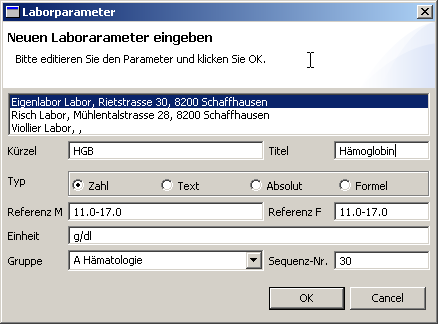
\includegraphics{images/labor1}
  \caption{Neues Labor-Item erstellen}
  \label{fig:labor1}
\end{center}
\end{figure}

 Fig.\ref{fig:labor1} montre un champ de dialogue pour la création d'un nouveau élément de laboratoire respectivement le changement d'un élément déjà existant. Tout en haut vous introduisez le nom du laboratoire qui fourni les résultats (Le laboratoire doit déjà être introduit dans la rubrique 'contacts'. Ce qui apparaît dans l'affichage de l'élément sont le sigle et le titre. Choisissez comme 'type'\textit{chiffre}, \textit{texte} (pour paramètres qui ne se laissent pas saisir en forme de chiffre comme par exemple un résultat bactériologique), \textit{absolu} fpour paramètres qui ne peuvent être que positive ou négative et \textit{formule} pour des résultats qui doivent être calculés (par exemple le cholestérol LDL selon la formule de Friedewald, chose qui est expliquée ci-après (\ref{ref:formel})).

 Sous\textit{RéférenceM} vous introduisez les valeurs de référence pour les hommes, sous \textit{RéférenceF} ceux pour les femmes \footnote{Elexis nécessite ces informations pour pouvoir marquer des résultats numériques automatiquement comme pathologique. C'est pourquoi il est indispensable que les valeurs de référence soient introduites comme 'de-à'.}, Sous\textit{unités} vous introduisez l'unité pour ce paramètre.

Sous \textit{groupe} vous déterminez dans quel groupe ce paramètre doit être classé. Des groupes déjà existants se trouvent déjà dans le Combo-Boxe et peuvent être facilement sélectionnés. Pour créer un nouveau groupe vous pouvez simplement introduire son nom. Le nom du groupe doit avoir le format suivant : 
une ou plusieurs lettres, un espace et ensuite un texte quelconque. Le préfixe décide sur l'ordre sur la feuille de labo de sorte que le groupe \textit{A Hématologie } se situe en dessus du groupe \textit{B Electrolytes } et \textit{DA Valeurs hépatiques } avant \textit{DC Valeurs rénales}. A vous de choisir la dénomination et l'ordre des groupes.

Sous\textit{no de séquence } vous décidez sur l'ordre dans le groupe càd où sera situé le paramètre spécifique à l'intérieur du groupe. Le no de séquence doit être un chiffre. La séquence des éléments est déterminée par le rapport de taille des chiffres. Nous conseillons de ne pas utiliser des chiffres très suivis pour pouvoir insérer plus tard encore quelques éléments si nécessaire.

\subsection{Valeurs de laboratoire calculées (Type Formule)}
\label{ref:formel}
\index{Formule}
\index{valeurs de laboratoire!formule}
Une valeur de labo du type  \textit{Formule} n'est pas introduite mais calculée par une formule quelconque. Normalement on se réfère à d'autres valeurs de labo déjà connues dont la valeur à calculer est dépendante. Prenons comme exemple la valeur du cholestérol LDL qui se calcule selon la formule de Friedewald. Cette formule nécessite comme paramètres les valeurs suivantes : Cholestérol totale, Triglycérides et Cholestérol HDL. La formule : \textit{Cholestérol totale -HDL-(TG/2.2)}. Pour notre exemple ces paramètres sont connus de façon suivante :
\begin{itemize}
  \item Cholestérol totale : Groupe  \textit{G Métabolisme des graisses }, No de séquence 10
  \item Cholestérol HDL : Groupe \textit{G Métabolisme des graisses }, No de séquence 20
  \item Triglycérides : Groupe \textit{G Métabolisme des graisses }, No de séquence 40
\end{itemize}

Nous créons maintenant un nouveau paramètre nommé  \textit{Cholestérol LDL (calculé)} dans le groupe G et nous lui donnons par exemple le No de séquence 21 (comme vous constatez, il était sage de laisser quelques plages libres dans la numérotation de la séquence)  (Fig. \ref{fig:labor2}).
%\usepackage{graphics} is needed for \includegraphics
\begin{figure}[htp]
\begin{center}
  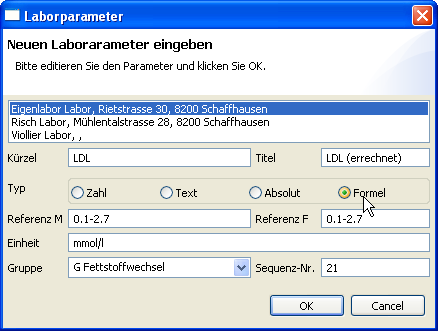
\includegraphics{images/labor2}
  \caption{Berechneten Laborwert erstellen}
  \label{fig:labor2}
\end{center}
\end{figure}
 Ensuite vous cliquez sur la désignation du type\textit{Formule}. et le dialogue pour l'introduction de la formule s'ouvre :\\
 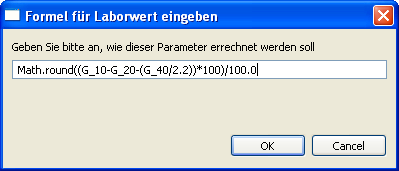
\includegraphics{images/labor3}\\
Pour nous référer dans la formule à d'autres valeurs de labo, nous utilisons leur indexe de groupe (donc ce qui se trouve devant l'espace dans le nom du groupe) et leur no de séquence séparés par un 'underscore'.  Pour le Cholestérol totale on utilise donc G\_20. La formule de Friedewald devient donc : \textit{G\_10-G\_20-(G\_40/2.2)}. Ceci donnerait une valeur de 9 chiffres, raison pour laquelle nous arrondissons la valeur avec Math.round à deux chiffres.

 Si les résultats de labo qui concernent la formule seront introduits Elexis essayera immédiatement de faire le calcul. Si ceci ne réussit pas, par exemple parce que certains résultats manquent encore, Elexis met \textit{?formel?} (voir Fig.  \ref{fig:labor4}).
 %\usepackage{graphics} is needed for \includegraphics
\begin{figure}[htp]
\begin{center}
  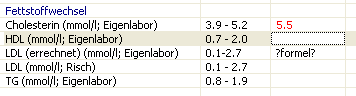
\includegraphics{images/labor4}
  \caption{Laboreintrag, noch nicht komplett}
  \label{fig:labor4}
\end{center}
\end{figure}

Seulement lorsque tout les valeurs nécessaires pour faire le calcul sont accessibles, la valeur du résultat sera affichée.  (Fig. \ref{fig:labor5}).
%\usepackage{graphics} is needed for \includegraphics
\begin{figure}[htp]
\begin{center}
  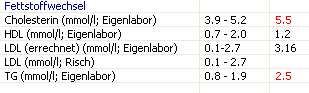
\includegraphics{images/labor5}
  \caption{Laboreintrag, komplettiert}
  \label{fig:labor5}
\end{center}
\end{figure}

\section{Codes de prestations}
Dépendant des différents Plugins qui concernent la facturation des prestations on trouve des différents codes. En Suisse nous avons à cet endroit normalement le tarif Tarmed et le tarif du Laboratoire. Des explications plus détaillées se trouvent à la page \pageref{arzttarife}.

\section{Traitement de texte}
Dans Elexis le traitement de texte pour des lettres etc. se définit par le choix des plugins càd on peut définir quel type de traitement de texte on veut choisir. Cependant, après avoir fait le choix il est déconseillé de changer ce réglage car s'il existent déjà quelques documents faits, on risque de ne plus pouvoir les ouvrir après un changement. Nous suggérons d'utiliser sous Windows le Plugin NOAText et sous Linux Office-Wrapper.
